\label{chap:arch}

\subsection{\textit{Hardware}}
Because not all sensors are designed to run at 1v8 up to 3v3, we need to be able to dynamically
change the operating voltage of the node. We used TPS62742, a step-down switching DC/DC converter
with up to 90\% efficiency, voltage selectable output from 1v8 to 3v2 with 200mV step, 360nA
quiescent current and a special mcu controllable load output, with push-pull transistors. In
inactive state the load line is pulled to GND and when active is pulled to VCC. When active it
consumes 12uA, but compared to the controlled sensors, this should not be noticeable. Because this
allows to completely power down the sensors, the "stand-by" current consumption is 0uA and it also
eliminates the previous design problem of floating GND which allowed the sensors to "steal" power
from other pins and not be properly disabled.

The node can be connected to an extension daughter board which fully respects the Arduino pinout.
This allows to easily test and prototype new configurations in order to be able to deliver the best
results in shortest time. Also existing hardware designed for Arduino can work with this board,
which increased the number of compatible hardware. In total, 20 I/O pins are available, pins that
can be used for connecting sensors, either on the daughter board, or directly on a specialty
designed board.

A jumper can select whether the Node is powered from USB or from other 2v1+ voltage supply or it can
be used for precise power measurement using an oscilloscope. In case the DC/DC converter is not
needed the node can use other power source.

\subsection{\textit{Performance}}

The SAMR21 micro-controller is an ARM cortex M0+ core clocked at 48 MHz with 32KB of RAM and 256KB
of flash. Being a 32-bit architecture and a new architecture, even though SAMR21 consumes 5.5mA
compared to 4.1mA of Atmega128RFA1, for simple 32-bit integer addition, SAMR21 consumes only 49nJ
per iteration while the 8-bit micro-controller consumes 274nJ, almost 5 times more. Considering
performance figures, SAMR21 was 9 times faster with 403950 iterations per second while
Atmega128RFA1 managed only 44890 iterations.

Testing the performance of branch predictor, revealed that the M0+ is only 12\% better than
the older 8-bit counterpart, but thanks to the frequency difference, it ends up being 3,36 times
faster.


\begin{figure}[ht] \centering
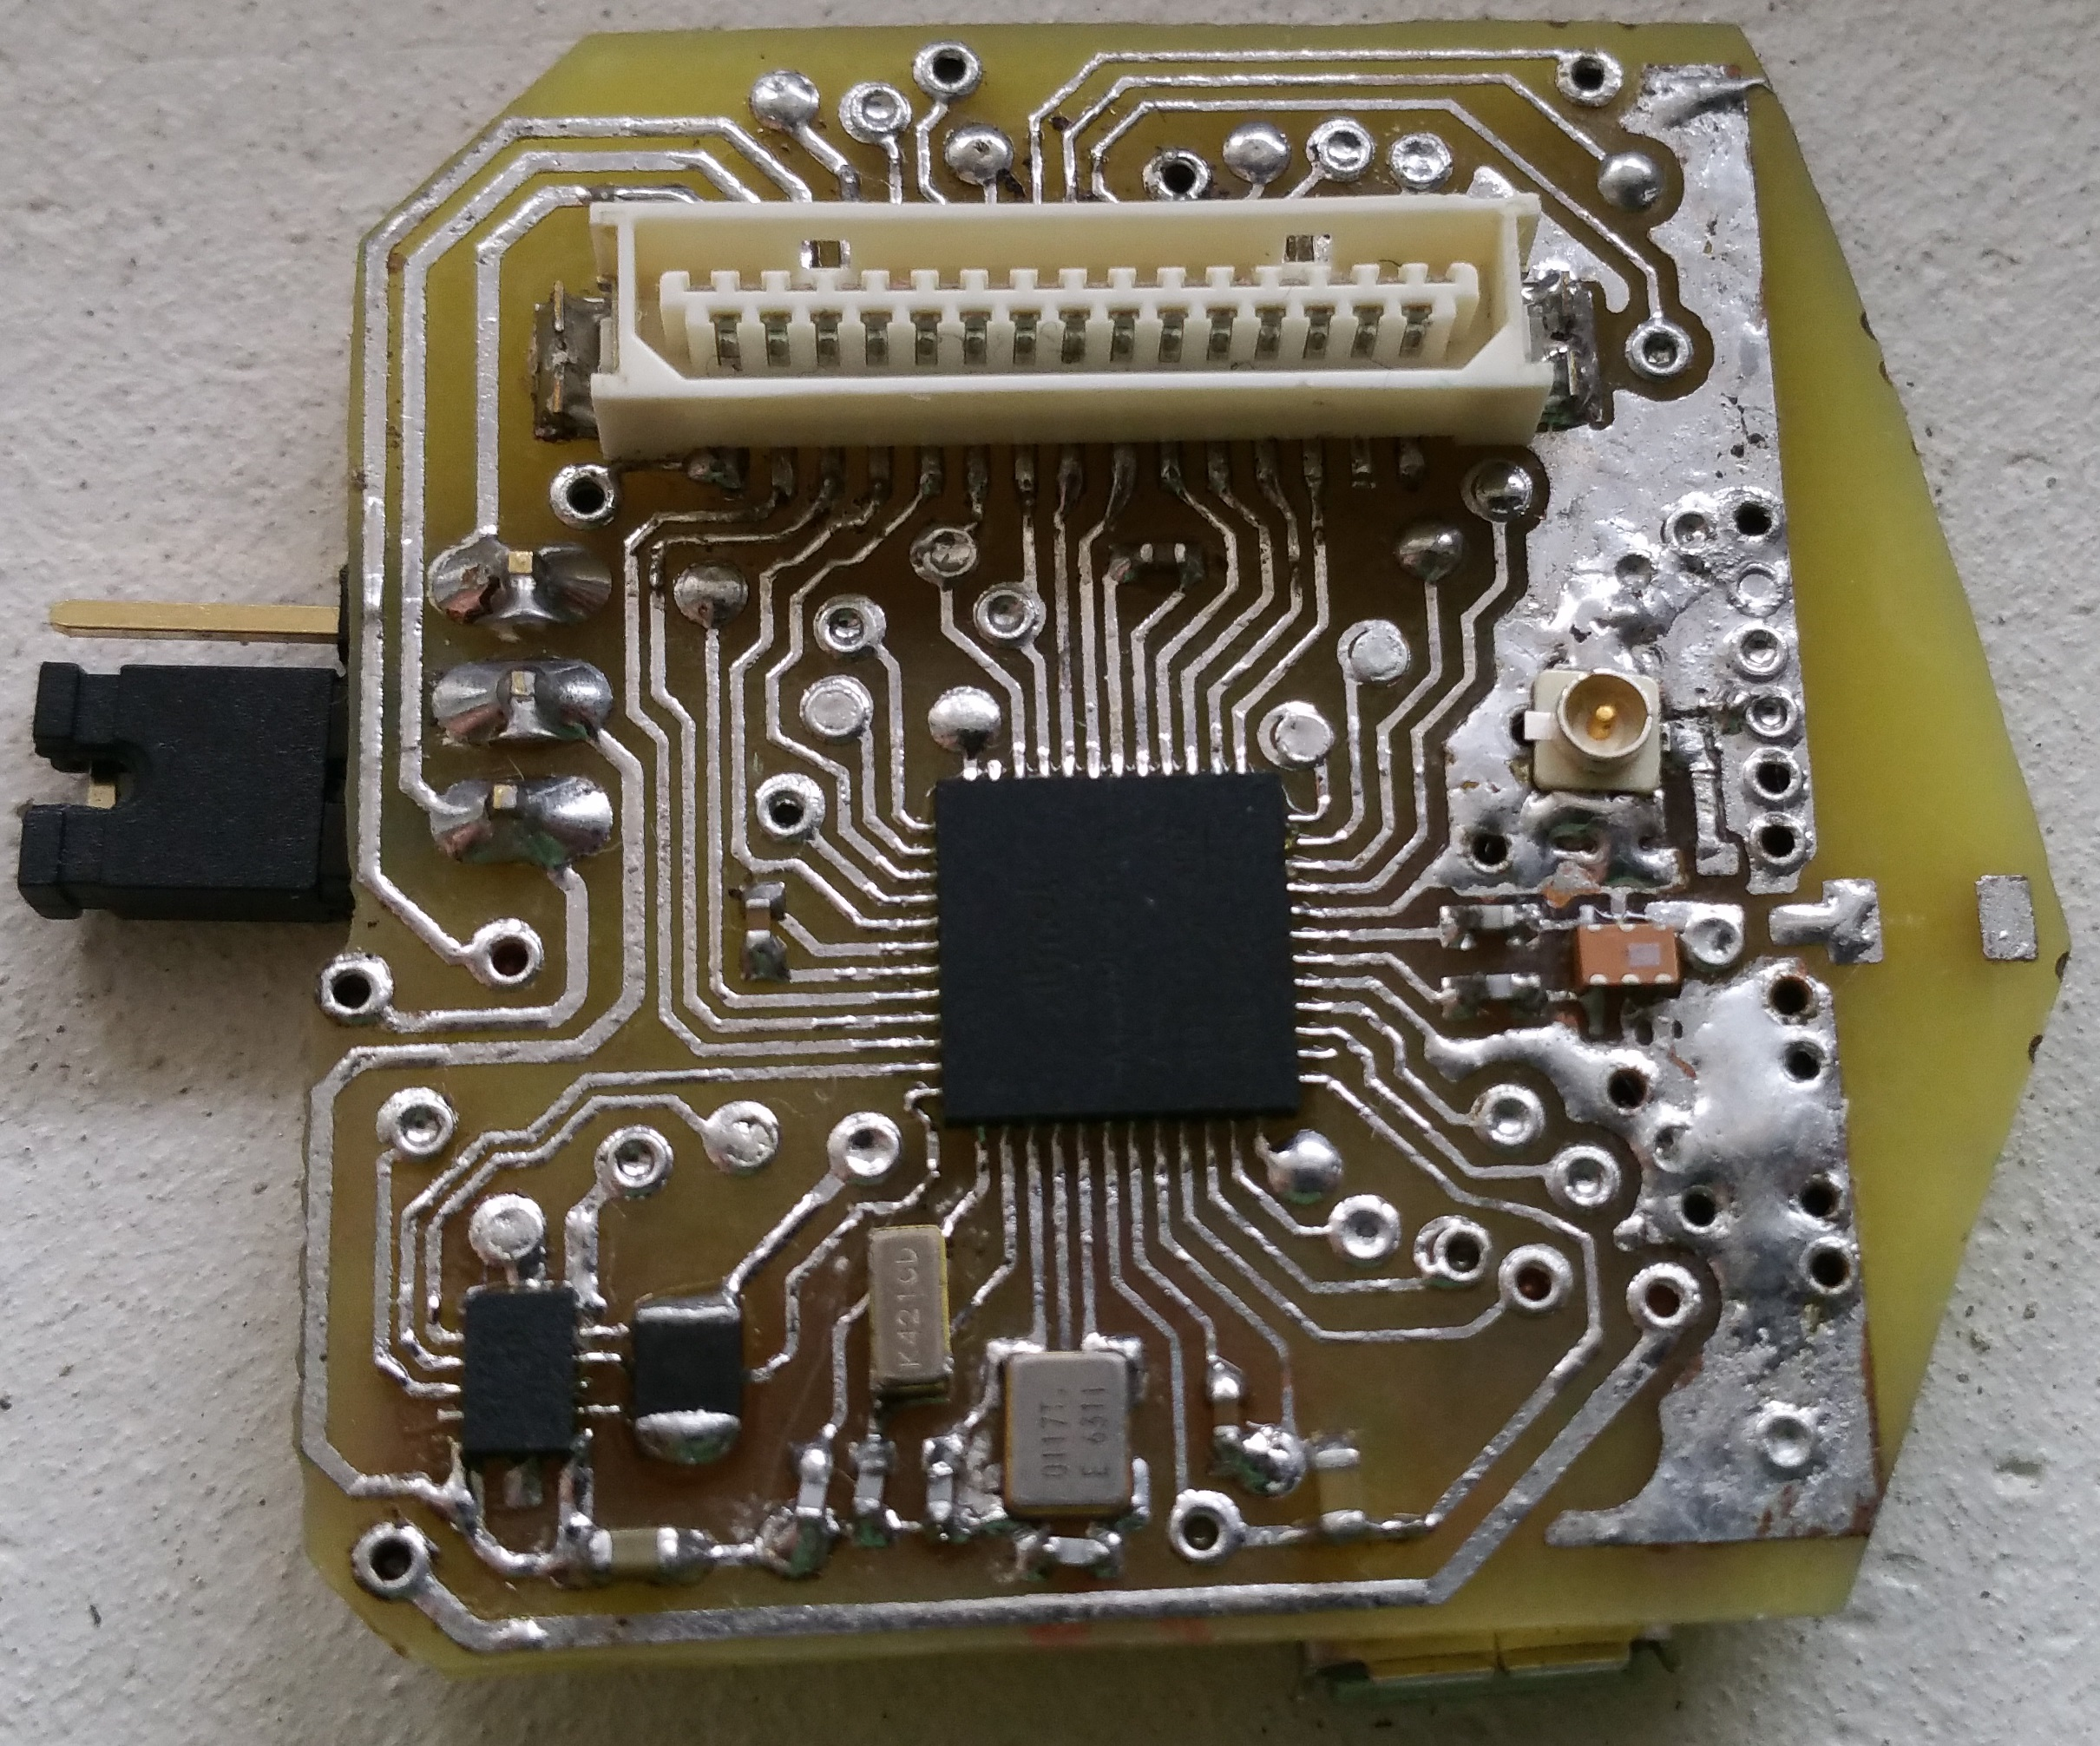
\includegraphics[width=0.5\textwidth]{img/sparrowrf.jpg}
\caption{Sparrow R node}
\end{figure}

The SAMR21 micro-controller is almost the same micro-controller as SAMD21, which is used in Arduino
Zero boards. Thanks to this, we could use exiting code, but unfortunately this does not mean well
written one.

Even thought the Arduino software is well designed, it was not designed with low power approach
from the beginning. We will describe some of the problems encountered when trying to create the software stack.

The first problem noticed was that the Arduino Zero board had no sleep functionality implemented.
The ideal idle current consumption should have been less than 5uA, tested and measured using a
project created in Atmel Studio 7.0. The current consumption of the board was around 350uA. We dig
deeper and discovered that the USB device was always initialized, witch accounted for the extra 200
uA. The rest of 150uA came from a default initializations of the pins as input pins, but this only
lowered the current consumption to about 60uA. We kept searching for a cause, and discovered that
the clock generators are never disabled at start-up, which accounted for about 30uA.

So far we managed to decrease the idle current consumption for the platform from 350uA to about
30uA @ 3v2, but still far from ideal. Surprisingly, lowering the voltage from 3v2 to 1v8 lead to a 3.3uA
sleep current consumption and when examining the power trace using a digital oscilloscope, we found
that very low frequency clock remains active, leading which at 3v2 leads to high spikes in power consumption.

Event tough we did not reach the goal of 5uA, we still reached a respectable 30uA @ 3v2 and less than 4 uA @1v8.
Due to the time constrains and the need to use the nodes in order to implement and test new
features, we decided that for now this is acceptable, and for future revisions, we will come back
and find the extra clock source.

Even the run current consumption was not ideal, instead of achieving the promised 70uA/MHz @ 3v2,
which would have lead to around 3.5mA current consumption of the CPU, the micro-controller
consumed 8mA @ 48MHz. We managed to reduce the current consumption to 5.5mA @ 48MHz, due to
clock optimizations presented bellow.

The peripheral interfaces are run at a much lower clock, instead of 48 MHz, we run them at 12 MHz.
Also if peripherals are not used, we completely disable them. Due to this, we ran into problems
related to SERCOM implementation, a generic module that handle USART, SPI and I2C. It was working
on Arduino Zero, because the CPU and the BUS were configured to run the same speed, but due to the
previous clock source modifications, the SERCOM did not set the correct speed. Also, there are 6
SERCOMs, and instead of enabling the clock for each one only when it is used, all of them were
enabled, which lead to extra power consumption during run time.

\begin{figure}[ht] \centering
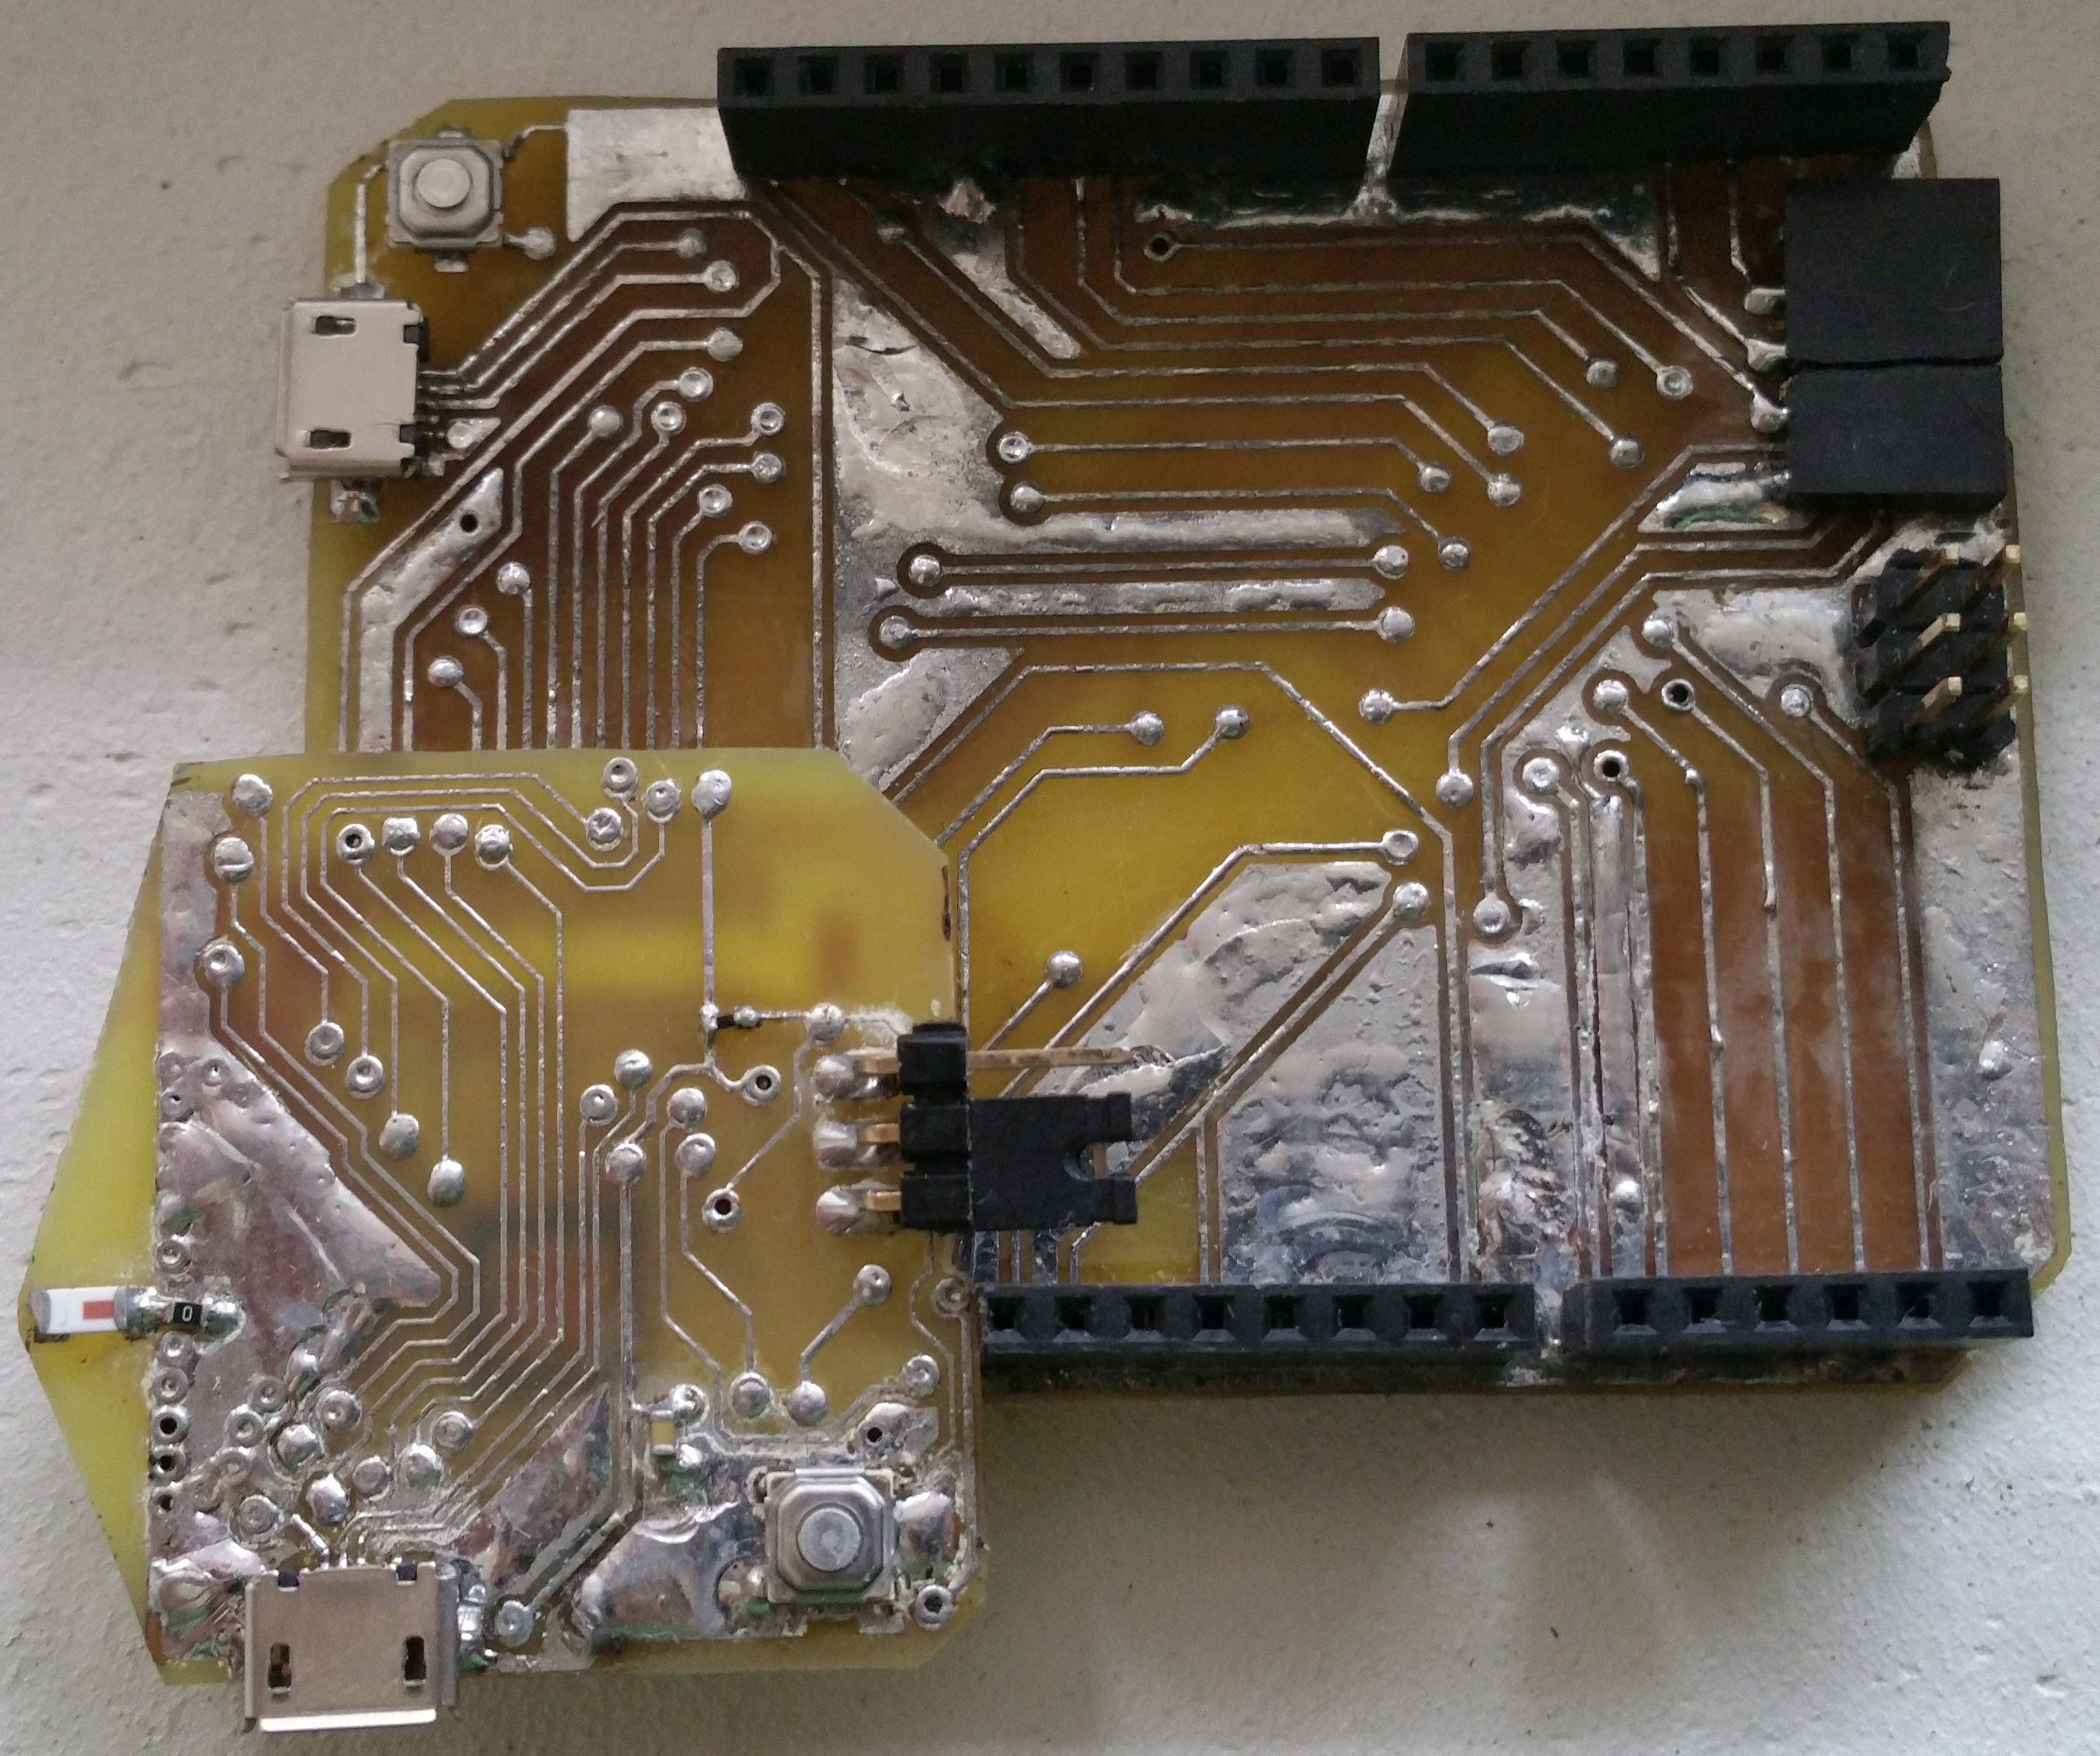
\includegraphics[width=0.5\textwidth]{img/base-with-sensor.jpg}
\caption{Sparrow R node mounted on Aduino compatible base}
\end{figure}
\subsection{\textit{Software}}


We implemented new modules designed for low power like sleep, power management which can dynamical
change the running voltage between 1v8 to 3v2 when requested and enable or disable the LOAD power
line. This allows the user to select which voltage is better required for applications. For example,
some sensor must be run at exactly 2v8 or other run at 2v5 or higher. This module allows for
precise voltage selection with 200mV increments, use the sensor, and then switch to the lowest
voltage in order to obtain the best power consumption possible.

The RF module is AT86RF233, integrated into the micro-controller. An exiting Arduino library
\cite{rf233}
exists for the RF but in order to add new features, we integrated the module for the RF in the core
of the platform, in order to let the user focus on what to do with the platform and not how to do
something with it. Also, extra futures and bug fixes are easier to be done if the module is
integrated in the platform. For example, in case the RF is constantly running in receive mode for
more than 5 minutes, it is recommended to do Fine Tuning of the PLL clock in order to eliminate
possible clock skews. Other feature is when the module automatically receives a packet, it saves it
locally together with RSSI and LQI, which can be later read and used buy the user. The internal
buffer is designed for 8 packets of 127KB of data, which amounts for 1 KB of ram. The buffer is
cyclic, so in case the buffer is not read, the oldest data is discarded and replaced by a new one.
This should not happen very often, because the buffer is large enough to handle all request, even
for high bandwidth transfers.

If the user has a need to save the data in case of power failure, the micro-controller has an
EEPROM like functionality which allows a 16KB region of flash to emulate EEPROM write endurance.
The flash contains pages of 64 bytes, and the EEPROM has an overhead of 4 bytes, which leaves 60
bytes for actual data. Also, for each page, another page must be reserved for further use.
The results is that out of 16KB used, the total amount of usable space left is $\frac{16*1024}{2}
* \frac{60}{64} = 7680 bytes$. This should be more than enough for normal use because the normal
endurance of 25k cycles of flash write and erase are increased to at least 150k, with typical
values reaching 600k cycles. If a new software is uploaded, the EEPROM zone is completely erased.

For timekeeping when sleeping, RTC functionality was implemented. Besides keeping the time, RTC
provides alarm interrupts for a special date, which can be configured to be triggered every
minute, every hour, every day, every month, every year, or only once. Together with another
peripheral named EventSys, periodic interrupts are provided and the interrupts interval can range
from once every second up to 128 times per second, with increments of power base 2.

Because the software and hardware are never perfect, a watchdog functionality is also implemented,
in order to avoid code lock-up or hardware failure due to extreme environment conditions.

